\section{Heuristic Based Scheduling}
\label{sec:simres}
\subsection{Heuristics}
\label{subsec:heuristics}
ILP can give an optimal indirection schedule but it is too slow to be used in real switch. To prove the practical benefits of indirection, we designed and implemented a scheduling algorithm based on simple heuristics. This algorithm runs in O(n) time complexity. N is the number of ports of the hybrid switch. With this algorithm, indirection schedule can be calculated in real switch in a short time. 

The core of our scheduling algorithm is the heuristics. Based on our observation on the optimal schedule provided by ILP and our understanding of the hybrid switch problem, we come up with the following heuristics:

\begin{enumerate}
  \item Indirection should increase the number of zero entries in each row of the demand matrix.
  \item Indirection should keep the variance of the number of zero entries in different rows low.
  \item Indirection should not add the max value of row/colum sum.
  \item Indirection should add few additional demands.
\end{enumerate}

These heuristics come from our observation and thinking. Heuristic 1 is the core reason why indirection can improve the performance of hybrid switch. By reducing the zero entry number in the demand matrix, the hybrid switch can have a higher chance to make a schedule that can take less configuration times. Reducing configuration times is the best benefit brought by indirection.

However, blindly reducing the zero entry number might not get good performance because the total time needed to serve the demand is largely determined by the worst row/column in the demand matrix. For each row, any non-zero entry will need one reconfiguration to serve the demand if it is not passed to packet switch. To make the tail better, we come up with our second heuristic. We want to make the zero entries to best fit the uniform distribution in the whole demand matrix.

For a specific row, the transmitting time for all its demand is configuration time plus the serving time. Serving time is determined by the sum of all its non-zero entries. So the max value of a row/column sum means the longest serving time in the demand matrix. As our heuristic is not able to optimize both the serving time and configuration time. We do not want to extend the max sum value to increase the serving time. That's our reasoning for heuristic 3.

Every indirection will increase the overall demand by an amount of the indirected volume. By placing those demand in surplus slots in one configuration and reduce the configuration time, indirection can improve performance. However, the indirection schedule generated by heuristic might not be an optimal one. So if we can reduce the zero entry without adding much demand, that will help the algorithm achieve better performance improvement. 

\subsection{Scheduling Algorithm}
\label{subsec:algorithm}
Our scheduling algorithm is based on the heuristics described in Section~\ref{subsec:heuristics}. It combines all the heuristics together. Pseudo code of the algorithm is shown below. 

{\tt \small
\begin{verbatim}
for i in range(iteration_numer):
    r := index of row with smallest zero number
    sum := 0
    for j in range(indirect_limit):
        s := index of the smallest non-zero entry in r
        t := chooseTarget(r, s) #  t is the index of the chose entry in r
        v := maxRecDemand(r, t) # v is the max demand (r, t) can receive
        schedule.add(v from (r, s) to (r, t))
        sum += v
    if sum >= m[r, s]:  #m[r, s] is the demand of entry (r, s)
        schedule.exec()
    else:
        schedule.restore()
\end{verbatim}
}

In this scheduling algorithm, we always start indirection in the row with fewest zero entries. As after indirection, that row will have one more zero entry, we are effectively reducing the variance of zero entry number in different rows. For the selected row, our algorithm will start with the smallest element. This way, it can add one more zero entry by just adding the smallest demand in that row. This is the smallest efforts to create one more zero entry. Our algorithm also guarantees that whenever it does indirection on an entry, it will make that element to an zero entry, or it will not do indirection on that entry. So every indirection will increase the zero entry number by one.

In the pseudo code, \emph{chooseTarget()} is an important function. The target it chooses will affect the performance of indirection much. In choosing this element, it first guarantees that the target (r, t) and its mirror position (t, r) which will also add demand because of indirection are non-zero entries. If they are zero entries, we will not be able to reduce zero entry number. How to choose a good target in the non zero entries is another problem needs investigation. Currently, we have two selection strategy, random selection and largest entry first selection. The thinking behind random selection is that it can best indirect demand uniformly to other entries. The reason of using largest entry first selection is that it can indirect small entries to large entries and those large entries would possibly be full and then fewer capacity will be wasted in one configuration transmission.


\subsection{Simulation Results}
To test our heuristics, we implemented the algorithm described in Section~\ref{subsec:algorithm} in the Solstice scheduling simulator~\cite{Liu:2014}. We did experiments using the simulator and compared the results of our algorithm with that of the Solstice scheduling algorithm.In our simulation experiments, the switch simulator has 64 ports. Each port will have a skewed demand matrix consists of 2 big demands and 30 small demands. The simulator will run for a pre-defined time and check how much demand is served by the hybrid switch. We will also compare the configuration times to see if indirection can effectively reduce it.

\begin{figure}
	\centering
	\begin{minipage}{3in}%
		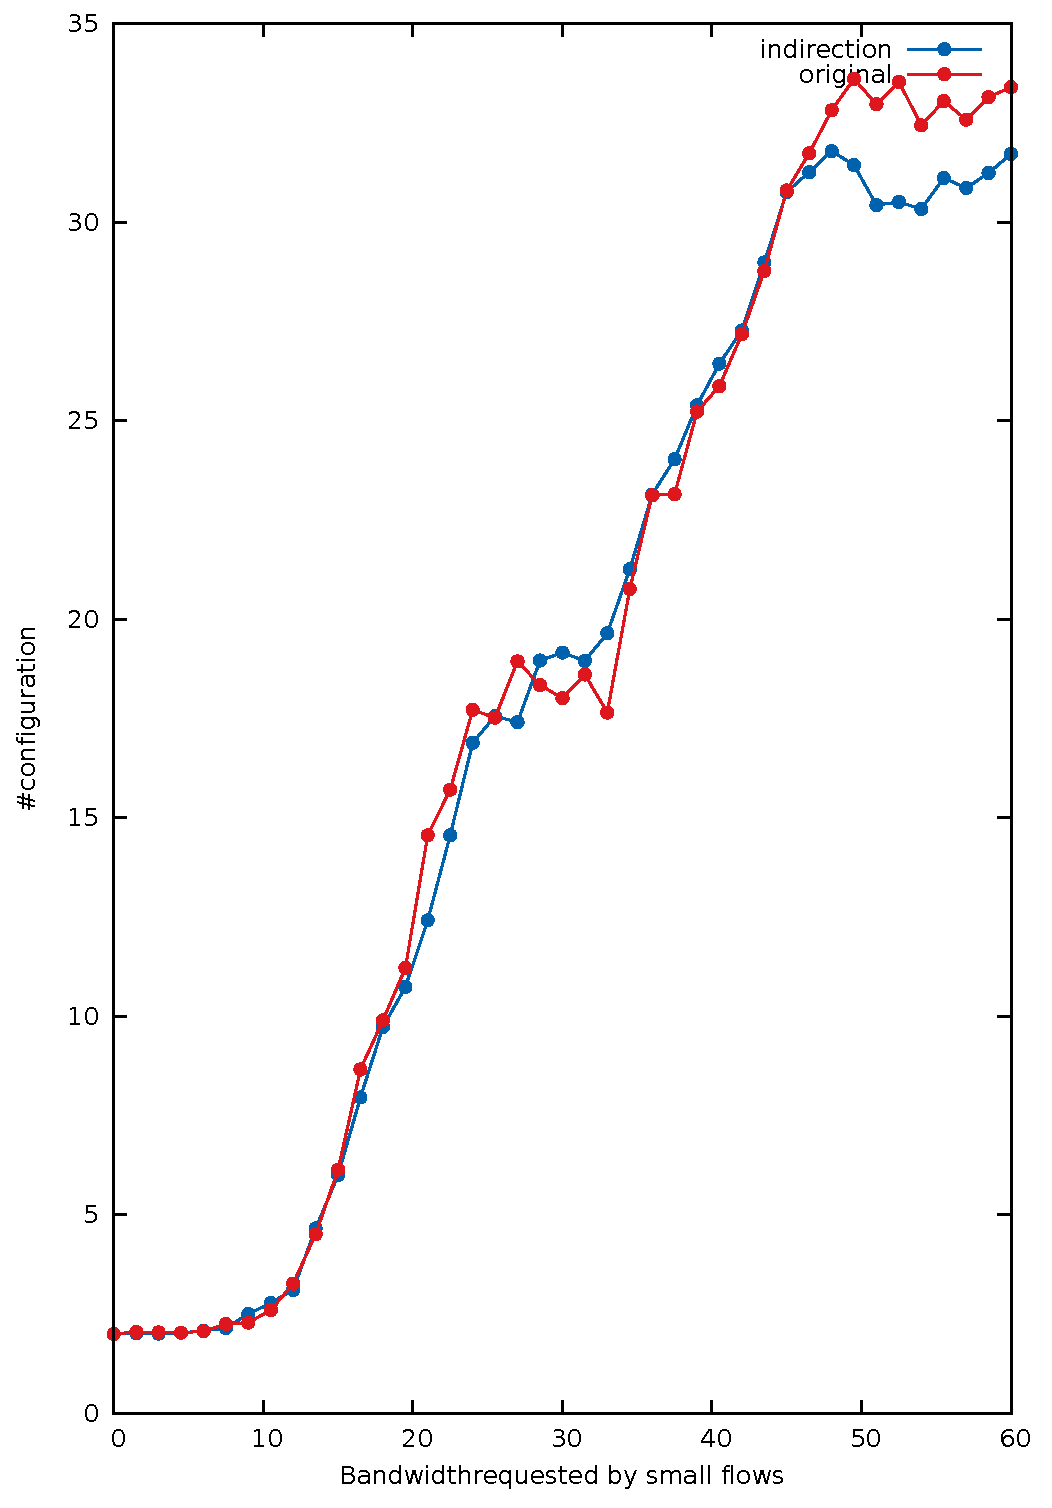
\includegraphics[width=3in]{figures/ndayRandom}
		\caption{Configuration number with random selection}
		\label{fig:ndayRandom}
	\end{minipage}%
	\qquad
	\begin{minipage}{3in}%
		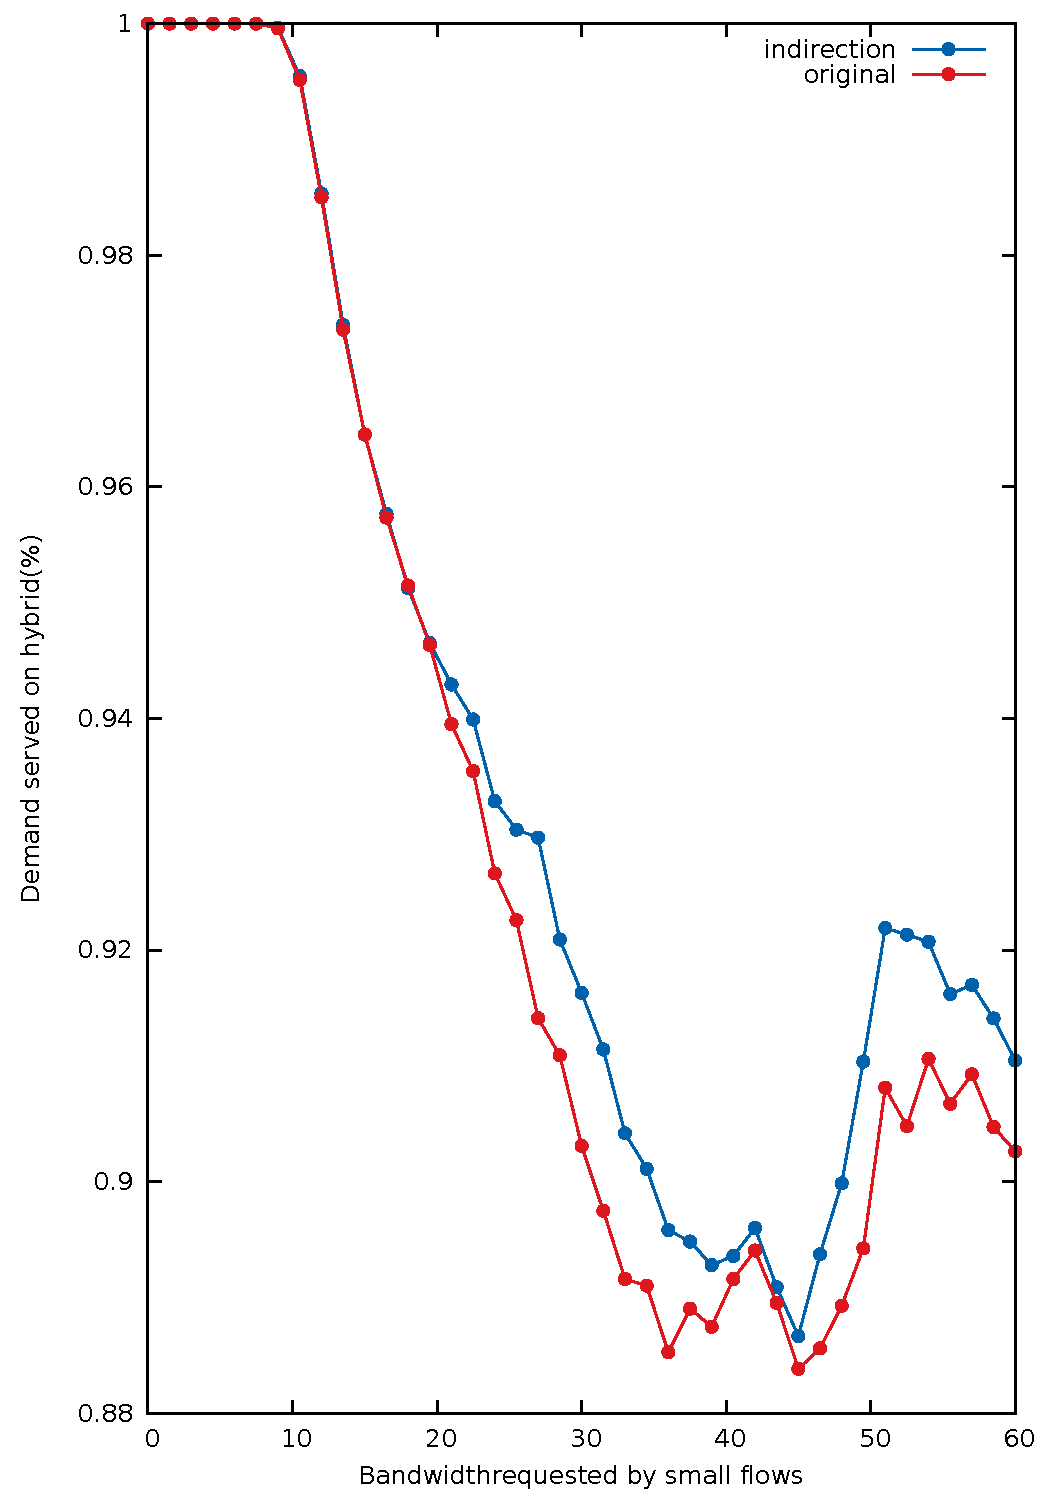
\includegraphics[width=3in]{figures/ndem3Random}
		\caption{Demand served by hybrid switch with random selection}
		\label{fig:ndem3Random}
	\end{minipage}%
\end{figure}

Figure~\ref{fig:ndayRandom} and Figure~\ref{fig:ndem3Random} are experiment result comparison on number of configuration and demand served by hybrid switch. Here we use the random target selection to pick indirection targets in the same row. The x axis of the two figures represents the percentage of demand in small demands. For example, x=30 means 30\% of the whole demand comes from small demands.

From the experiment results we can see that when more demands come from small demands, indirection algorithm can effectively reduce configuration times. When x > 45, the reduction is about 3 configuration times. As a result, more demand can be served on hybrid switch because less time is used on configuration and more time can be used to serve demands. This experiments shows that with simple heuristics, indirection can effectively improve the hybrid switch performance. When x is bigger than 45, 1 - 2 percent more demand can be served on hybrid switch using indirection. The absolute increase is not significant but if we consider that 90\% of the demand has already been served by hybrid switch by using Solstice algorithm, the relative improvement is reasonable.

\begin{figure}
	\centering
	\begin{minipage}{3in}%
		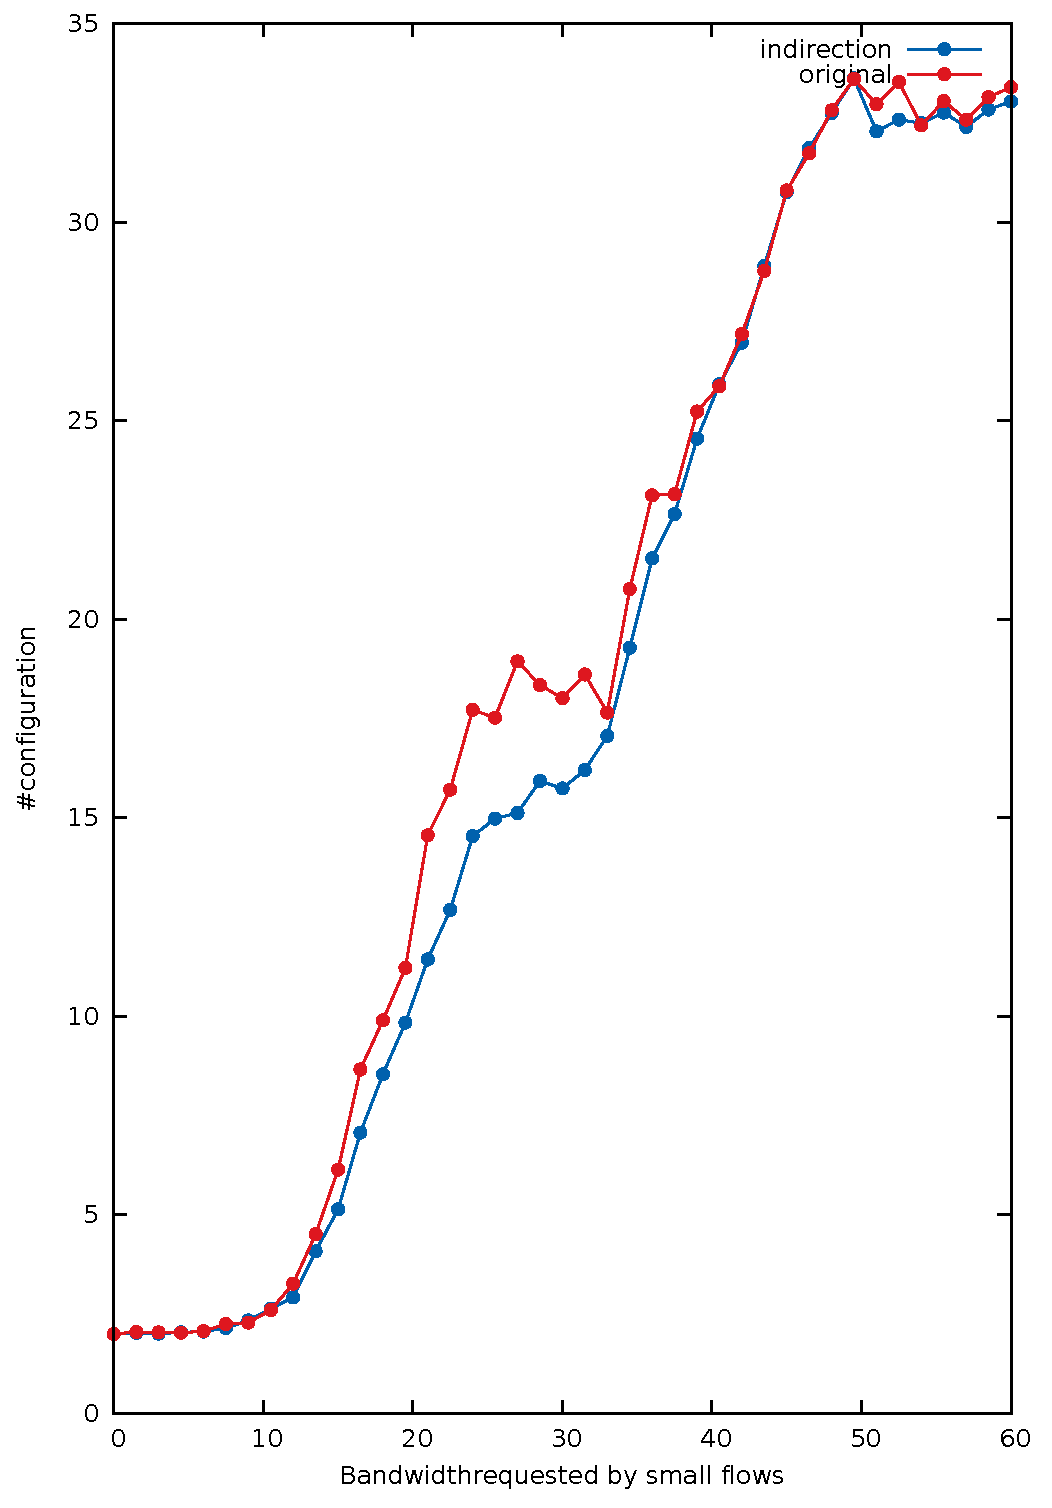
\includegraphics[width=3in]{figures/ndaySorted}
		\caption{Configuration number with largest entry first selection}
		\label{fig:ndaySorted}
	\end{minipage}%
	\qquad
	\begin{minipage}{3in}%
		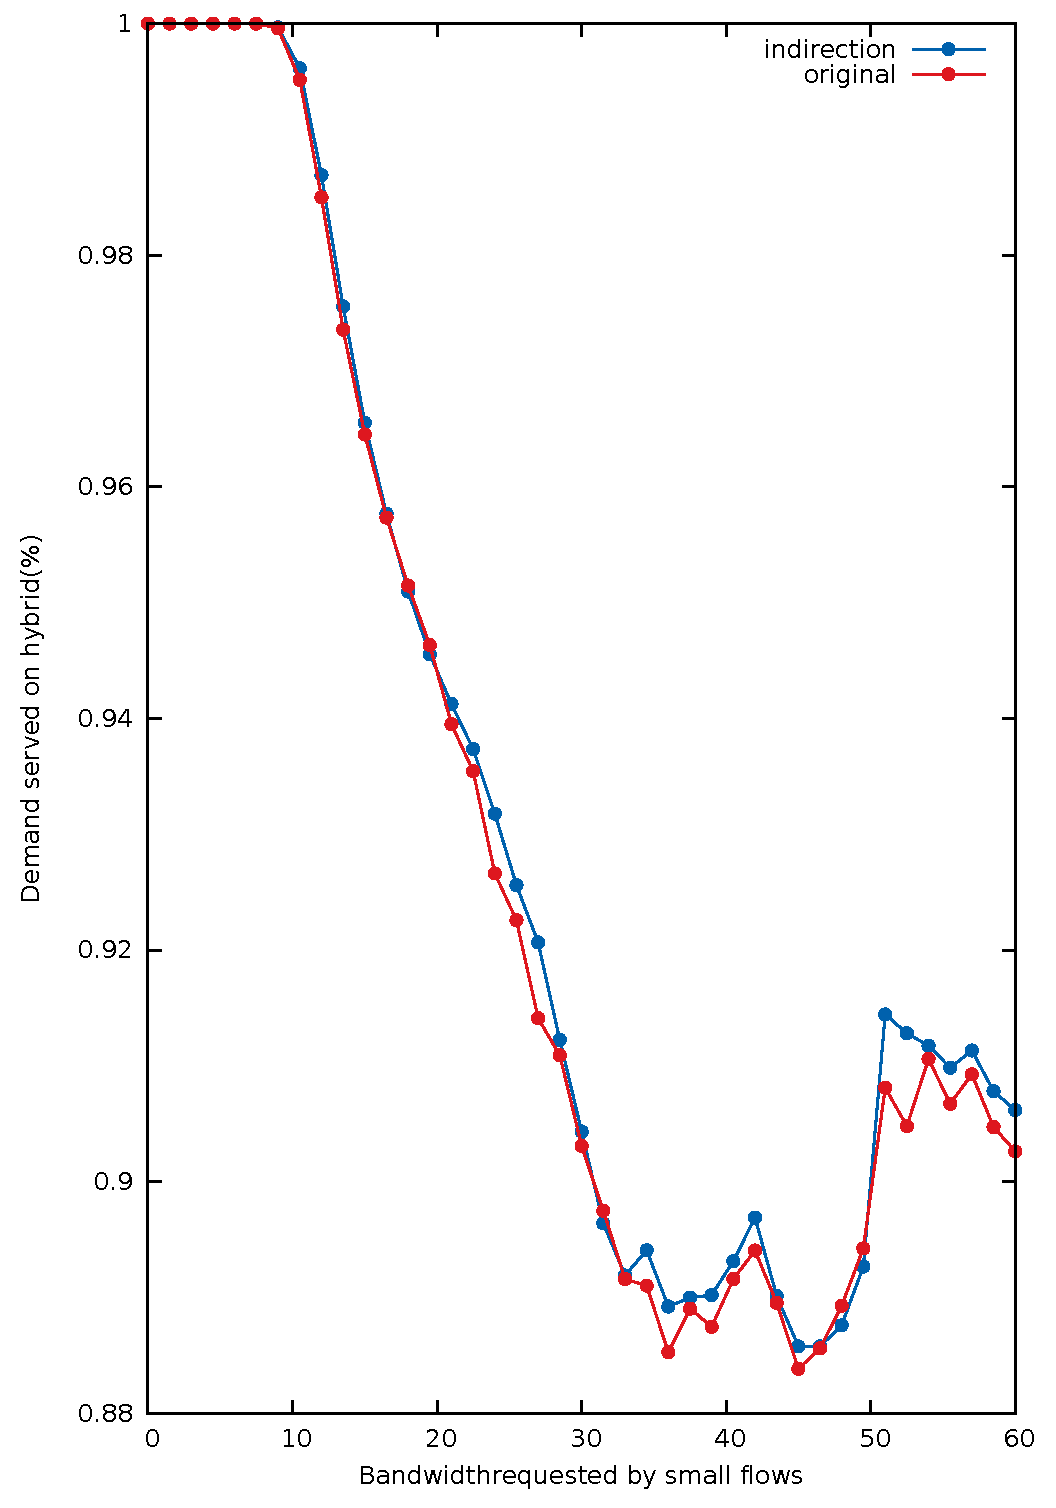
\includegraphics[width=3in]{figures/ndem3Sorted}
		\caption{Demand served by hybrid switch with largest entry first selection}
		\label{fig:ndem3Sorted}
	\end{minipage}%
\end{figure}

Figure~\ref{fig:ndaySorted} and Figure~\ref{fig:ndem3Sorted} are experiment result comparison with Solstice and indirection with largest entry first selection. We just change the selection strategy in the scheduling algorithm but the figure shape differs a lot from the previous experiment. When x is very large (e.g. x > 45), indirection does not see great advantages to the Solstice scheduling algorithm. But in the previous experiments with random selection, we do see improvements there. The improvements of using largest entry first in in the middle part. That is because large entries are filled up when about 30\% of demand come from small demands. Then few demand can be indirected to large entries. 

